\documentclass[9pt,xcolor=table]{beamer}
\usepackage[latin1]{inputenc}
\usepackage[english]{babel}
% \usepackage{graphics}
\usepackage{graphicx}
\usepackage{hyperref}
\usepackage{units}
\usepackage{amsmath}
\usepackage{amsfonts}
\usepackage{amssymb}
\usepackage{color, colortbl}
\usepackage{amsmath}
\usepackage{wrapfig}
\usepackage[normalem]{ulem}
\usepackage{multirow}
\usepackage{verbments}

\usetheme{MPICBG}

\def\cpp{\texttt{C++}}
\def\cpu{\texttt{CPU}}
\def\gpu{\texttt{GPGPU}}
\def\Cuda{\texttt{CUDA}}


\AtBeginSection[] 
{
\begin{frame}<beamer>
\frametitle{Outline}
\vspace{-1.5\baselineskip}
\begin{columns}[t]
  \begin{column}{.1\textwidth}
    \hfill
  \end{column}
  \begin{column}{.75\textwidth}
    \huge
    \tableofcontents[currentsection,hideallsubsections]
  \end{column}
  \begin{column}{.1\textwidth}
    \hfill
  \end{column}
\end{columns}
\end{frame}
}
   
\begin{document}
     
\pgfdeclareimage[height=1.5cm]{MPIlogo}{img/CBGlogo}
\titlegraphic{ \pgfuseimage{MPIlogo}  }
 
 
\title[PerfVsDesign]{Performance Versus Design}
\subtitle{- Advanced Programming School 2014 -}
\author[P. Steinbach]{Peter Steinbach}
\date{}
\institute[MPI CBG]{Max Planck Institute of Molecular Cell Biology and Genetics\\Scientific Computing Facility}
\addtocounter{framenumber}{-1}
\renewcommand*\inserttotalframenumber{XX} 

 
{
\setbeamertemplate{footline}{} 
\maketitle
}

\begin{frame}[t]
\frametitle{Outline}
\vspace{-1.5\baselineskip}
\begin{columns}[t]
  \begin{column}{.1\textwidth}
    \hfill
  \end{column}
  \begin{column}{.75\textwidth}
    \huge
    \tableofcontents[hideallsubsections]
  \end{column}
  \begin{column}{.1\textwidth}
    \hfill
  \end{column}
\end{columns}
\end{frame}

\section[Why \cpp{}?]{Why \cpp{}?}
\begin{frame}
\frametitle{\insertsection{}}
\begin{block}{A Devil's Advocate Game}
  \Huge
  \begin{center}
    \alert{Why \cpp{}?}
  \end{center}
\end{block}
\end{frame}

\subsection{My view}
\begin{frame}[c]
\frametitle{\insertsectionhead{} : \insertsubsection}
\vspace{-1.\baselineskip}
\begin{columns}[t]
  \begin{column}{.48\textwidth}
    \begin{exampleblock}{Pros}
      \begin{itemize}
      \item
      \end{itemize}
    \end{exampleblock}
  \end{column}
  \begin{column}{.48\textwidth}
    \begin{alertblock}{Cons}
      \begin{itemize}
      \item
      \end{itemize}
    \end{alertblock}
  \end{column}
\end{columns}
\end{frame}

\part{Performance}
%\section[Performance]{Performance}
\section{A Definition}
\begin{frame}
\frametitle{\insertsectionhead{} : \insertpart{}
}
\vfill
\begin{block}{Etymology}
  \begin{description}
  \item[perform] from Middle English \textit{performen}, \textit{parfournen} (``to perform''), from Anglo-Norman \textit{performer}, \textit{parfourmer}, alteration of Old French \textit{parfornir}, \textit{parfurnir} (``to complete, accomplish, perform''), from \textit{par}- + \textit{fornir}, \textit{furnir} (``to accomplish, furnish''), \dots
  \item[ance] added to the stem of a verb to form a noun indicating a state or condition, such as result or capacity, associated with the verb.\\
    \begin{flushright}
      \small(\href{http://en.wiktionary.org/wiki/perform}{wiktionary})
    \end{flushright}

  \end{description}
\end{block}
\vfill
\begin{block}{Computer Performance}
  \begin{center}
    \dots is characterized by the amount of useful work accomplished by a computer system or computer network compared to the time and resources used.\\
  \end{center}
  \begin{flushright}
    \small(\href{http://en.wikipedia.org/wiki/Computer_performance}{wikipedia})
  \end{flushright}

  \end{block}
\vfill
\end{frame}

\section[Resources]{The resources available}
\subsection{Computers?}
\begin{frame}[c]
\frametitle{\insertsectionhead{}: \insertsubsection{}}
\begin{figure}[htb]
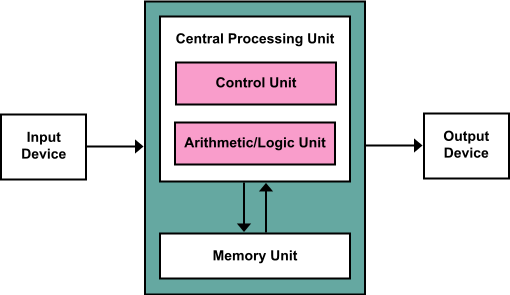
\includegraphics[height=0.65\textheight]{img/Von_Neumann_Architecture}\\[12pt]\Large
Stored-Program Computer Architecture (\cite{VonNeumann}, source: \href{http://en.wikipedia.org/wiki/Von_Neumann_architecture}{wikipedia})
\end{figure}
\end{frame}

\subsection{From Source To Instruction}
\begin{frame}
\frametitle{\insertsectionhead{}: \insertsubsection{}}
\end{frame}

\subsection{From Disk to Memory}
\begin{frame}
\frametitle{\insertsectionhead{}: \insertsubsection{}}
\end{frame}


\section[Measurement]{The time needed}
\subsection{\texttt{time}}
\begin{frame}
\frametitle{\insertsectionhead{}: \insertsubsectionhead{}}
\end{frame}

\subsection{\texttt{perf}}
\begin{frame}
\frametitle{\insertsectionhead{}: \insertsubsectionhead{}}
\end{frame}

\subsection{\texttt{valgrind}}
\begin{frame}
\frametitle{\insertsectionhead{}: \insertsubsectionhead{}}
\end{frame}


\part{Tour de Force}
\section{The Blessings of Design}
\subsection{Inheritance}
\begin{frame}
\frametitle{\insertsectionhead{}: \insertsubsectionhead{}}
\end{frame}

\subsection{Over-Objectivism}
\begin{frame}
\frametitle{\insertsectionhead{}: \insertsubsectionhead{}}
\end{frame}

\subsection{Take-Home}
\begin{frame}
\frametitle{\insertsectionhead{}: \insertsubsectionhead{}}
\end{frame}

\section{The Free Lunch}
\section{Real-Life HPC}


\part{Exercises}
\section{Tasks}
\section{Results}

\section{Literature}
\begin{frame}[c]
\frametitle{\insertsection{}}
\nocite{*}
\tiny%footnotesize
\bibliographystyle{ieeetr}
\bibliography{slides}
\end{frame}

\end{document}




